\documentclass[../main.tex]{subfiles}

\begin{document}

    \begin{figure}[H]
        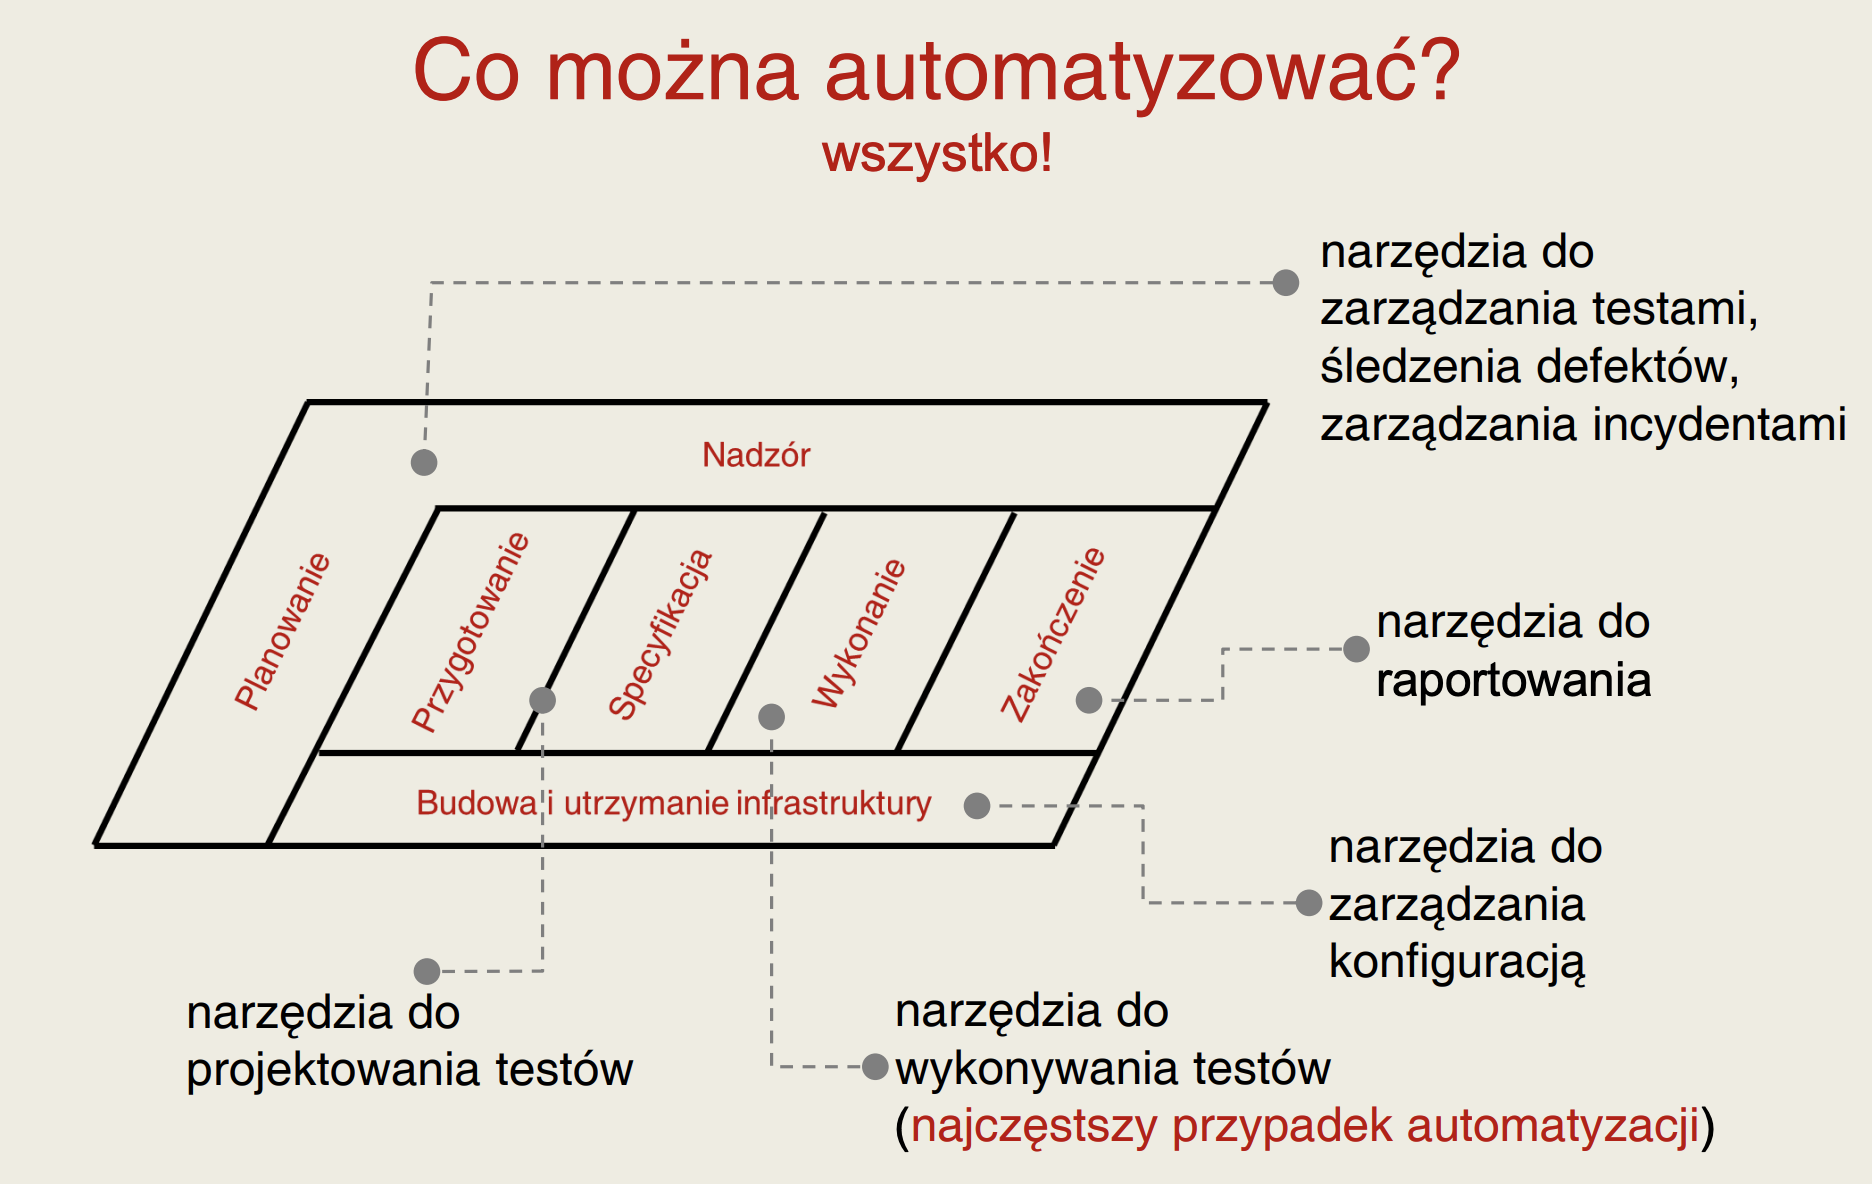
\includegraphics[width=\linewidth]{automatyzacja.png}
    \end{figure}

    \begin{figure}[H]
        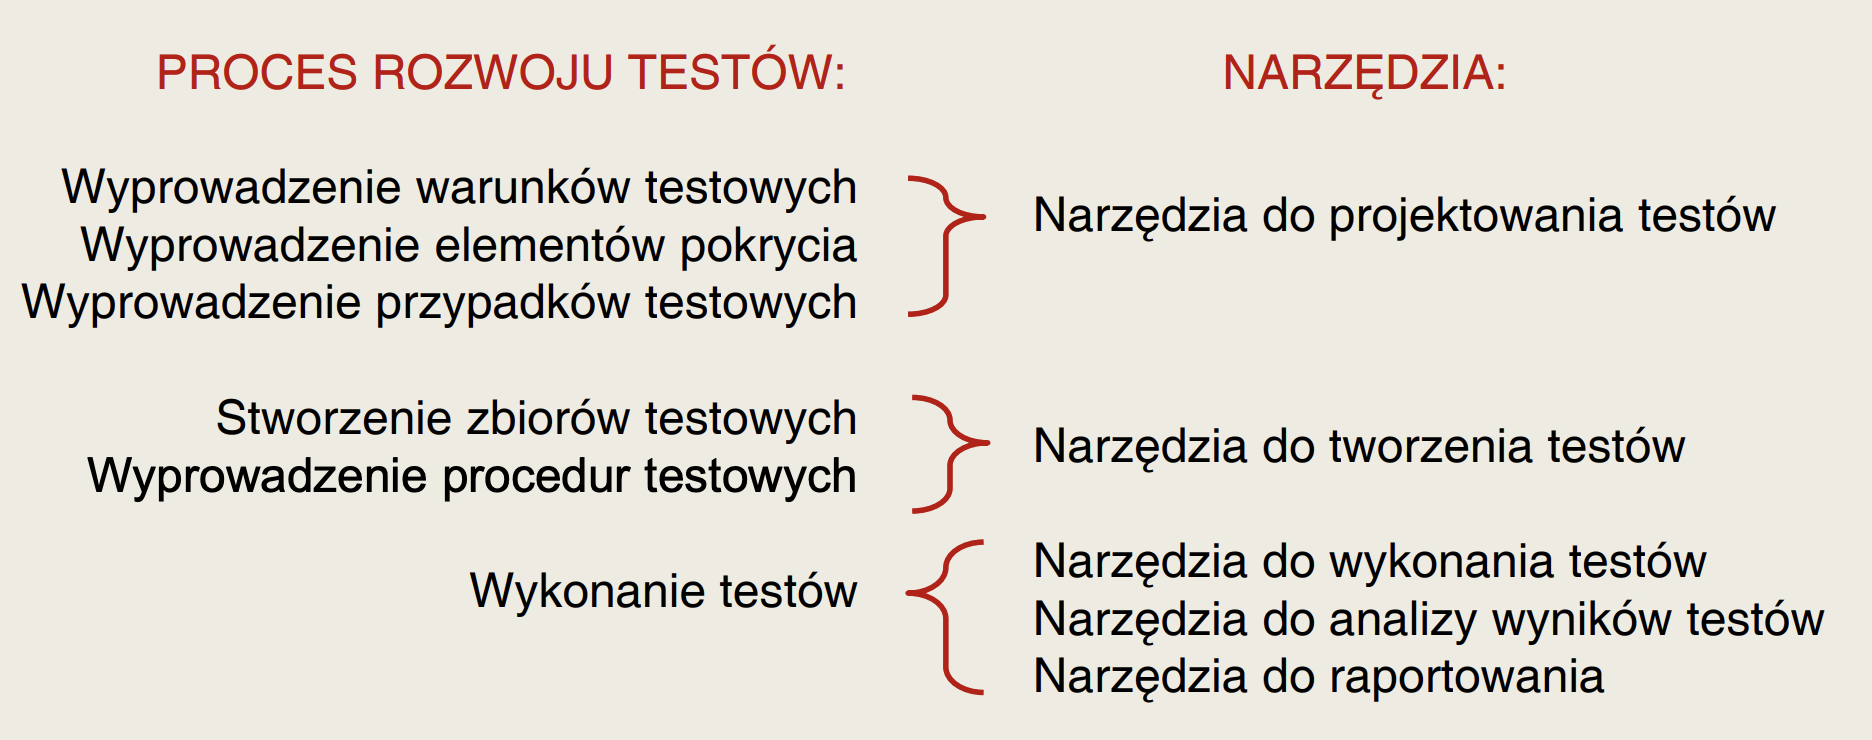
\includegraphics[width=\linewidth]{auttest.png}
    \end{figure}

    Przykładowe \textbf{cele i korzyści}
    \begin{itemize}
        \item wykonywanie testów przez uruchamianie skryptów
        \begin{itemize}
            \item powtarzalność, spójność, efektywność
        \end{itemize}
        \item wykonywane testów niemożliwych do wykonania ręcznego
        \begin{itemize}
            \item np. testy wydajności, analiza statyczna
        \end{itemize}
        \item automatyczne projektowanie testów
        \begin{itemize}
            \item np. testy oparte na modelu
        \end{itemize}
        \item pomiar, analiza i raportowanie metryk
        \begin{itemize}
            \item powtarzalność, spójność, obiektywność pomiaru
        \end{itemize}
        \item automatyczna generacja danych testowych
        \begin{itemize}
            \item często nietrywialna
        \end{itemize}
        \item porównywanie wyników rzeczywistych z oczekiwanymi
        \begin{itemize}
            \item często nietrywialne
        \end{itemize}
    \end{itemize}

    Przykładowe ryzyka
    \begin{itemize}
        \item nierealistyczne oczekiwania
        \begin{itemize}
            \item „narzędzie zrobi wszystko”
        \end{itemize}
        \item niedoszacowanie
        \begin{itemize}
            \item kosztu, czasu, pracochłonności wstępnego wdrożenia
            \item czasu i pracochłonności do osiągnięcia znaczących korzyści
            \item pracochłonności utrzymania generowanych artefaktów
        \end{itemize}
        \item zbytnie poleganie na narzędziu
        \begin{itemize}
            \item „narzędzie się nie myli”
        \end{itemize}
        \item niewykorzystanie kontroli wersji
        \begin{itemize}
            \item bałagan, chaos, błędy związane z zarządzaniem konfiguracją
        \end{itemize}
        \item zależności i problemy ze współpracą krytycznych narzędzi
        \item słaba reakcja dostawcy
        \begin{itemize}
            \item brak wsparcia, szkoleń itp.
        \end{itemize}
    \end{itemize}


    \textbf{Efekt próbnika (probe effect)}
    Niektóre narzędzia są inwazyjne, tzn. mogą wpływać na rzeczywisty wynik testu. To zjawisko nazywa się
    efektem próbnika.

    Efekt próbnika = niezamierzony wpływ na zachowanie systemu spowodowany pomiarami tego systemu.

    Przykład 1: w profilowaniu kodu i pomiarach wydajności opóźnienia spowodowane wykonaniem
    instrumentowanego kodu mogą skutkować niepoprawnym lub nieprzewidywalnym działaniem.

    Przykład 2: czas działania może być inny ze względu na dodatkowe instrukcje wykonywane przez narzędzie,
    albo może to skutkować innymi metrykami pokrycia.

    \begin{figure}[H]
        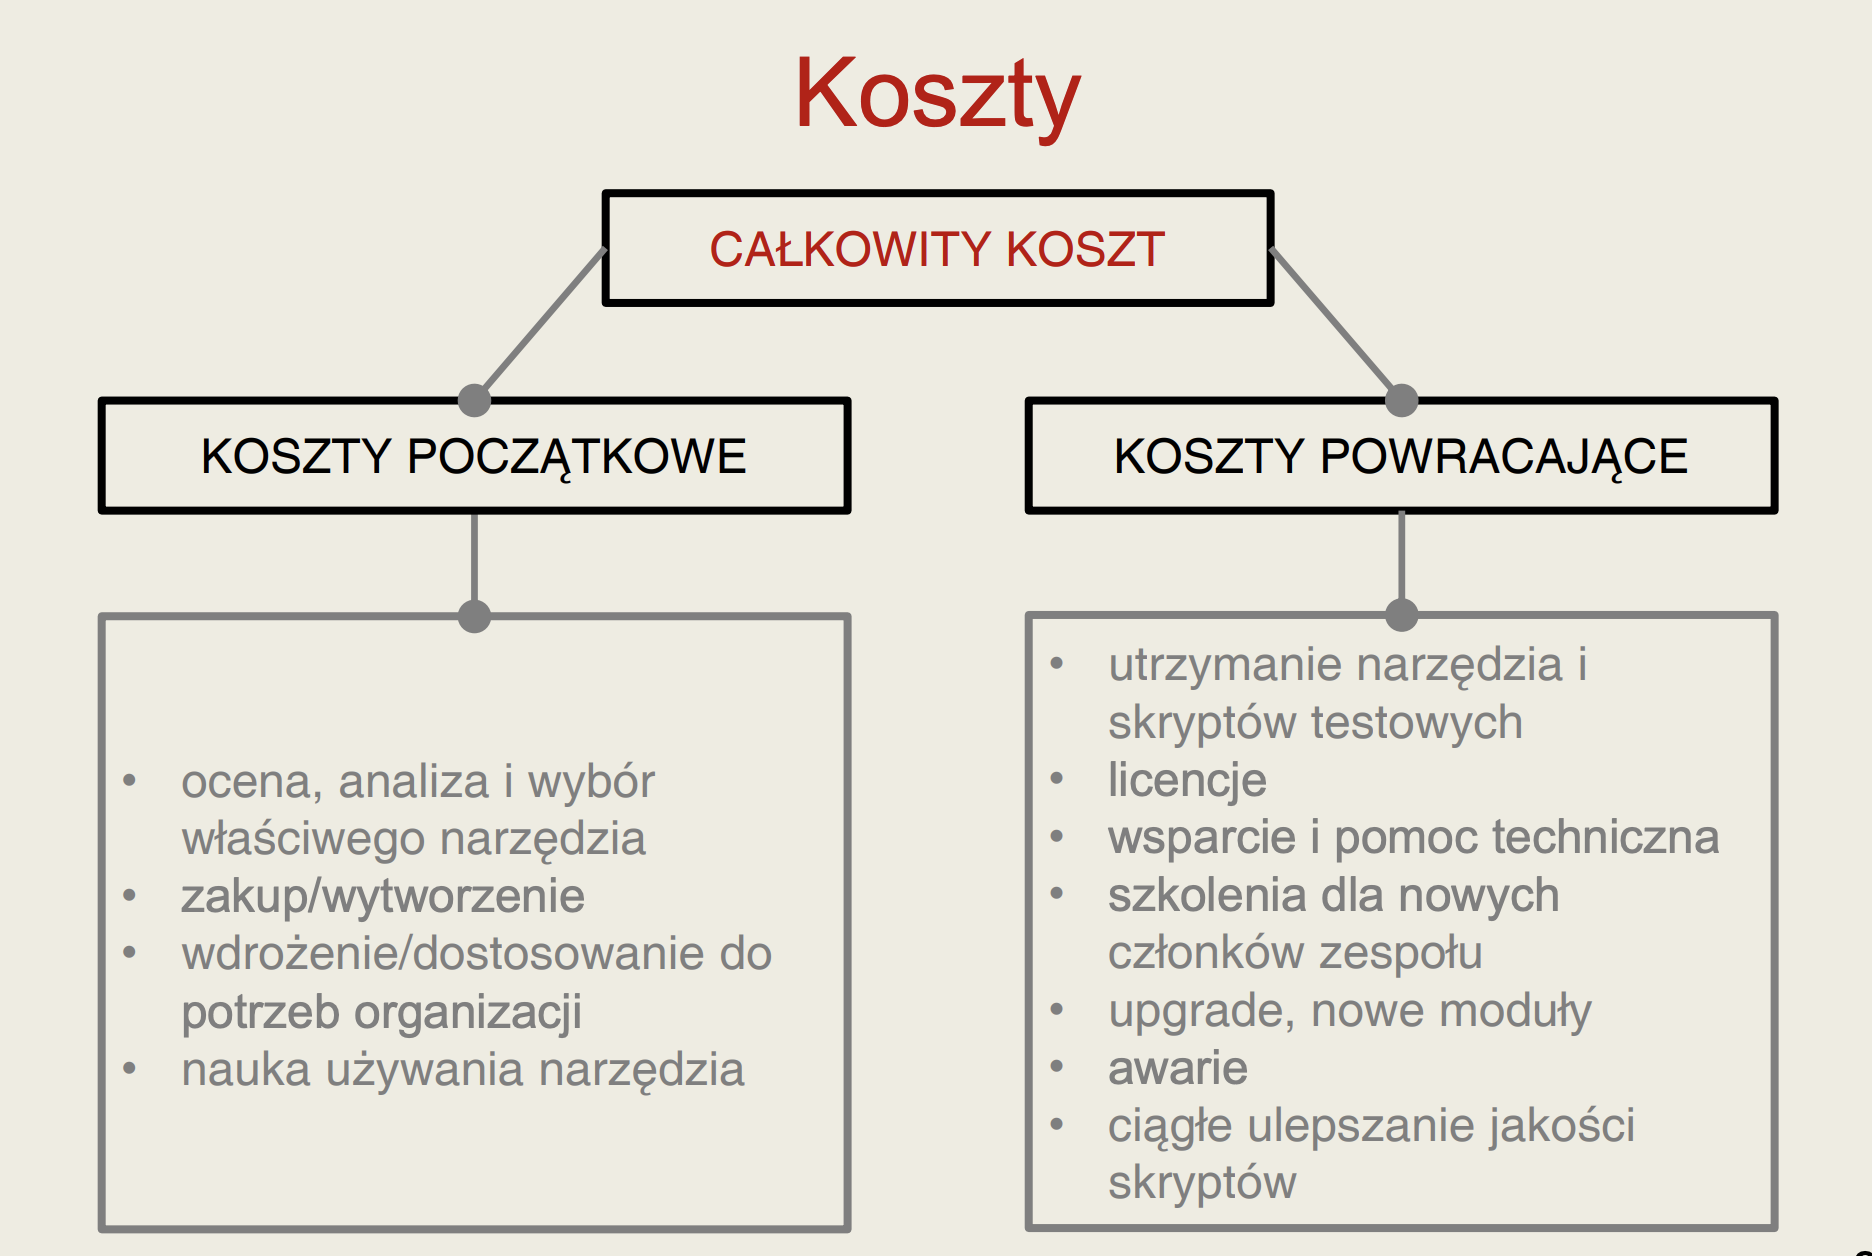
\includegraphics[width=\linewidth]{kosztaut.png}
    \end{figure}

    \subsection{ Generyczna architektura automatyzacji testów}
    \begin{figure}[H]
        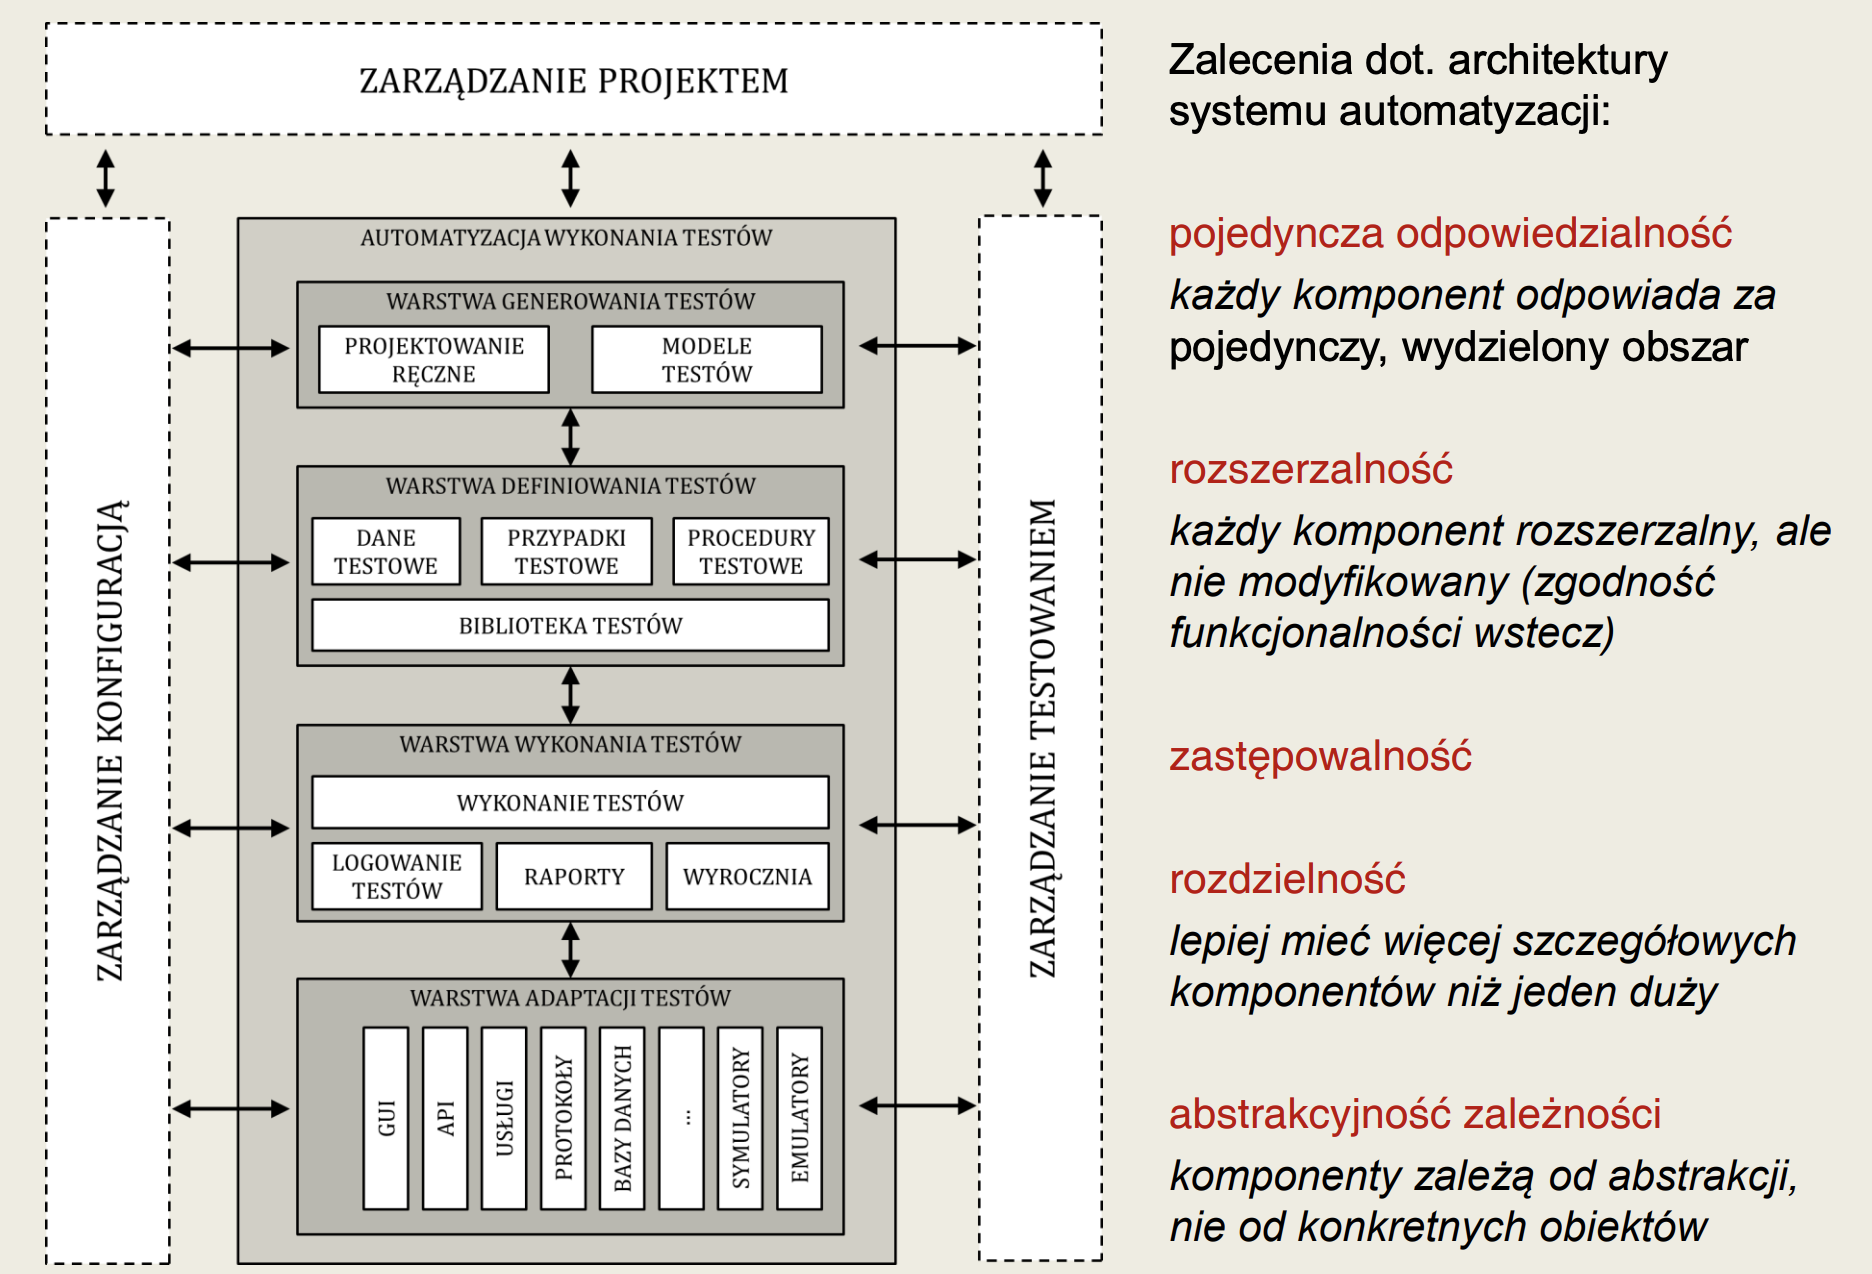
\includegraphics[width=\linewidth]{genaut.png}
    \end{figure}

    \subsection{Automatyczna generacja danych testowych}
    \begin{itemize}
        \item metoda losowa
        \item generacja z rozkładu prawdopodobieństwa
        \item generacja z modelu
        \item generacja na podstawie symbolicznego wykonania kodu
        \item generacja metodyczna (np. pair-wise)
        \item generacja na podstawie danych zewnętrzych
    \end{itemize}

    \subsection{Techniki automatyzacji testów}
    \begin{tabular}{ p{5cm} | p {5cm} | p{5cm} }
        \textbf{Technika} & \textbf{Zalety} & \textbf{Wady}\\
        \hline

        \textbf{nagraj i odtwórz} &
        stosowalne na poziomie GUI lub API,
        łatwe do konfiguracji i użycia, nie
        wymaga znajomości języków
        &
        trudne w utrzymaniu, problemy
        gdy potrzeba czasu na
        odpowiedź systemu\\
        \hline
        \textbf{skrypty linearne} &
        brak żmudnych i kosztownych
        przygotowań, znajomość
        programowania niekonieczna gdy
        skrypt tworzony automatycznie
        &
        koszt automatyzacji liniowy ze
        względu na liczbę skryptów;
        trudne i kosztowne w utrzymaniu\\
        \hline
        \textbf{skrypty zorganizowane} &
        redukcja kosztów utrzymania,
        zmniejszenie kosztu automatyzacji
        nowych testów
        &
        zwiększone koszty początkowe
        tworzenia reużywalnych
        skryptów; wymaga umiejętności
        programowania\\
        \hline
        \textbf{Data-Driven Testing} &
        niski koszt dodania testu; nie wymaga
        znajomości programowania; tanie w
        utrzymaniu
        &
        ograniczona możliwość
        przeprowadzania testów
        negatywnych\\
        \hline
        \textbf{    Keyword-Driven Testing} &
        tanie w utrzymaniu; swoboda w
        tworzeniu testów
        &
        kosztowna implementacja słów
        kluczowych; trudność w doborze
        właściwych słów\\
    \end{tabular}

    \subsection{Testowanie oparte na modelu}
    \begin{itemize}
        \item Testowanie oparte na modelu (MBT) to technika wykorzystująca modele do testowania
        \item Rozszerza i wspiera inne techniki, takie jak np. formalne techniki projektowania testów
        \item Podstawowa idea: ulepszyć jakość i efektywność projektu i implementacji testów przez
        \begin{itemize}
            \item projekt wyczerpującego (comprehensive) modelu MBT, zwykle z użyciem narzędzi, opartego na celach projektu testowego
            \item użycie modelu jako specyfikacji projektu testów, pozwalającego na automatyczną generację przypadków testowych z modelu
        \end{itemize}

        \item Główna motywacja: \textbf{efektywność}
        \begin{itemize}
            \item \textbf{komunikacja} - modelowanie ułatwia lepszą
            komunikację z interesariuszami
            \item \textbf{zrozumienie} - lepsza komunikacja pomaga stworzyć wspólną
            płaszczyznę zrozumienia wymagań w danej dziedzinie i uniknąć potencjalnych nieporozumień
            \item \textbf{łatwiejsze zaangażowanie} - w przypadku graficznych modeli MBT interesariusze
            (np. analitycy) mogą być zaangażowani wcześnie
            \item \textbf{ciągła poprawa kompetencji} - modelowanie wspiera to
            u testerów w danej dziedzinie
            \item \textbf{łatwa identyfikacja „problematycznych” części systemu} - dzięki abstrakcji modeli MBT
            \item \textbf{wczesna generacja i analiza przypadków testowych} - możliwe przed stworzeniem systemu
        \end{itemize}

        \item Główna motywacja: \textbf{wydajność}
        \begin{itemize}
            \item \textbf{wczesne unikanie defektów} - dzięki wczesnemu modelowaniu, modele
            mogą być dzielone z interesariuszami by weryfikowali wymagania
            \item \textbf{możliwe reużycie} - artefakty MBT z poprzednich projektów
            mogą być użyte do kolejnych projektów testów
            \item \textbf{automatyzacja} - np. generacja testaliów; redukcja defektów które można
            wprowadzić gdy testalia są tworzone i utrzymywane ręcznie
            \item \textbf{adaptacja do zmian} - różne suity testów mogą być generowane z tego samego modelu
            \item \textbf{uniwersalne modele} - MBT może być użyty do różnych celów testowania i do pokrycia
            różnych poziomów i typów testów
            \item \textbf{redukcja kosztów przy zmianie wymagań} - MBT pomaga zredukować koszty utrzymania gdy
            zmieniają się wymagania, bo model MBT dostarcza „single point of maintenance”
        \end{itemize}

        \item \textbf{Rodzaje modeli}:
        \begin{itemize}
            \item strukturalne
            \item behawioralne
            \item danych
        \end{itemize}
    \end{itemize}

    \textbf{Kryteria wyboru testów}:
    \begin{itemize}
        \item \textbf{Oparte na pokryciu}
        \begin{itemize}
            \item \textbf{Wymagania połączone z modelem} - wymaga, by elementy modelu były połączone z wybranymi
            wymaganiami. Pełne pokrycie wymagań odpowiada zestawowi testów całkowicie pokrywających wybrany zbiór wymagań
            \item \textbf{Elementy modelu MBT} - bazuje na wewnętrznej strukturze modelu. Definiuje się elementy
            pokrycia, a testy powinny je pokrywać. Przykłady elementów pokrycia:
            \begin{itemize}
                \item stany, przejścia, decyzje w diagramach stanów
                \item aktywności i bramki w modelach procesów biznesowych
                \item warunki i akcje w tablicach decyzyjnych
                \item instrukcje i warunki w modelach tekstualnych
            \end{itemize}
            \item \textbf{Oparte na danych} - związane są z takimi technikami projektowania testów jak:
            \begin{itemize}
                \item podział na klasy równoważności
                \item analiza wartości brzegowych
                \item heurystyki typu testy kombinatoryczne (np. pair-wise)
            \end{itemize}
        \end{itemize}
        \item \textbf{Inne}
        \begin{itemize}
            \item \textbf{Losowe} - Kryterium polega na losowym przechodzeniu przez model, w podejściu losowym przejścia są równo
            prawdopodobne. W podejściu stochastycznym wybór oparty o rozkład prawdopodobieństwa. Model reprezentuje profil
            użycia (tzw. \textbf{profil operacyjny}).
            \item \textbf{Oparte na scenariuszu/wzorcu} - Scenariuszem może być use case lub
            scenariusz użycia; wzorzec = częściowo zdefiniowany scenariusz, który można
            zastosować do modelu MBT aby wyprowadzić jeden lub wiele testów.
            \item \textbf{Sterowane projektem} - Podejście oparte na dodatkowej informacji projektowej, która została
            dodana do modelu aby wspierać zarządzanie testami i/lub aby osiągnąć specificzne cele testowe w projekcie.
            Informacje te to w szczeólności np. ryzyka, priorytety, wymagania na sprzęt testowy lub inne aspekty ważne dla projektu.
            Wybór przypadków testowych wymagających określonego sprzętu testowego odpowiada zastosowaniu kryterium opartego na projekcie.
        \end{itemize}
    \end{itemize}

    \subsection{Wdrażanie narzędzi w organizacji}
    \begin{itemize}
        \item ocena dojrzałości organizacji, mocnych i słabych stron
        \item ocena wg jasnych wymagań i obiektywnych kryteriów
        \item wykonanie dowodu słuszności pomysłu (proof-of-concept
        \item ocena dostawcy (w tym: szkolenia, wsparcie techniczne, aspekty komercyjne) lub firm udzielających wsparcia
        \item identyfikacja wymagań wewnętrzych na doradztwo i szkolenia
        \item ocena potrzeb szkoleniowych z uwzględnieniem obecnych umiejętności automatyzacji testów przez zespół testowy
        \item szacowanie stosunku korzyści do kosztów na podstawie konkretnego przypadku biznesowego
    \end{itemize}

    \subsubsection{Projekt pilotażowy}
    Wdrażanie wybranego narzędzia zaczyna się od
    projektu pilotażowego. Jego cele:
    \begin{itemize}
        \item szczegółowe zaznajomienie się z narzędziem
        \item ocena dopasowania narzędzia do obowiązujących procesów i praktyk, ustalenie co należałoby zmienić
        \item ustalenie standardów użycia, zarządzania, przechowywania, pielęgnacji narzędzia i artefaktów testowych (np. konwencja nazewnictwa plików)
        \item ocena, czy korzyści zostaną osiągnięte przy rozsądnych kosztach
    \end{itemize}

    Czynniki sukcesu:
    \begin{itemize}
        \item stopniowe wdrażanie narzędzia w pozostałej części organizacji
        \item adaptacja i doskonalenie procesu tak, by pasował do narzędzia
        \item zapewnienie szkoleń i doradztwa nowym użytkownikom
        \item zdefiniowanie wytycznych co do użycia narzędzia
        \item wdrożenie sposobu na zbieranie informacji z wykorzystania narzędzia
        \item monitorowanie wykorzystania narzędzia
        \item monitorowanie osiąganych korzyści
        \item zapewnienie wsparcia dla zespołu testowego w użyciu danego narzędzia
        \item zbieranie wniosków z wykorzystania narzędzia
    \end{itemize}
\end{document}